%%% LaTeX Template: Two column article
%%%
%%% Source: http://www.howtotex.com/
%%% Feel free to distribute this template, but please keep to referal to http://www.howtotex.com/ here.
%%% Date: February 2011

%%% Preamble
\documentclass[	DIV=calc,%
							paper=a4,%
							fontsize=12pt,%
							onecolumn]{scrartcl}	 					% KOMA-article class

\usepackage{lipsum}													% Package to create dummy text
\usepackage[brazil]{babel}										% English language/hyphenation
\usepackage[protrusion=true,expansion=true]{microtype}				% Better typography
\usepackage{amsmath,amsfonts,amsthm}					% Math packages
\usepackage[pdftex]{graphicx}									% Enable pdflatex
\usepackage[svgnames]{xcolor}									% Enabling colors by their 'svgnames'
\usepackage[hang, small,labelfont=bf,up,textfont=it,up]{caption}	% Custom captions under/above floats
\usepackage{epstopdf}												% Converts .eps to .pdf
\usepackage{subfig}													% Subfigures
\usepackage{booktabs}												% Nicer tables
\usepackage{fix-cm}													% Custom fontsizes
\usepackage[utf8]{inputenc}
\usepackage[top=2.5cm, bottom=2.5cm, left=2.5cm, right=2.5cm]{geometry}
\usepackage[ddmmyyyy]{datetime}
\addto\captionsenglish{%
	\renewcommand\tablename{Tabela}
	\renewcommand\figurename{Figura}
} 
 

 
%%% Custom sectioning (sectsty package)
\usepackage{sectsty}													% Custom sectioning (see below)
\allsectionsfont{%															% Change font of al section commands
	\usefont{OT1}{phv}{b}{n}%										% bch-b-n: CharterBT-Bold font
	}

\sectionfont{%																% Change font of \section command
	\usefont{OT1}{phv}{b}{n}%										% bch-b-n: CharterBT-Bold font
	}



%%% Headers and footers
\usepackage{fancyhdr}												% Needed to define custom headers/footers
	\pagestyle{fancy}														% Enabling the custom headers/footers
\usepackage{lastpage}	

% Header (empty)
\lhead{}
\chead{}
\rhead{}
% Footer (you may change this to your own needs)

%% ====================================
%% ====================================
%% mude o rodape  do projeto
%% ====================================
%% ====================================

\lfoot{\footnotesize \texttt{Template para entrega de texto} \textbullet ~Modelo de projeto}


\cfoot{}
\rfoot{\footnotesize página \thepage\ de \pageref{LastPage}}	% "Page 1 of 2"
\renewcommand{\headrulewidth}{0.0pt}
\renewcommand{\footrulewidth}{0.4pt}



%%% Creating an initial of the very first character of the content
\usepackage{lettrine}
\newcommand{\initial}[1]{%
     \lettrine[lines=3,lhang=0.3,nindent=0em]{
     				\color{DarkGoldenrod}
     				{\textsf{#1}}}{}}



%%% Title, author and date metadata
\usepackage{titling}															% For custom titles

\newcommand{\HorRule}{\color{DarkGoldenrod}%			% Creating a horizontal rule
									  	\rule{\linewidth}{1pt}%
										}

\pretitle{\vspace{-30pt} \begin{flushleft} \HorRule 
				\fontsize{50}{50} \usefont{OT1}{phv}{b}{n} \color{DarkRed} \selectfont 
				}

\title{Processo de produção de sofware pra saúde}		% Title of your article goes here

%% ====================================



\posttitle{\par\end{flushleft}\vskip 0.5em}

\preauthor{\begin{flushleft}
					\large \lineskip 0.5em \usefont{OT1}{phv}{b}{sl} \color{DarkRed}}
\author{Eduardo Amaral Pereira }  	% Author name goes here


\postauthor{\footnotesize \usefont{OT1}{phv}{m}{sl} \color{Black} 
					\\Universidade Tecnológica Federal do Paraná - Câmpus Cornélio Procópio 								% Institution of author
					\par\end{flushleft}\HorRule}

\date{}																				% No date


%%% Begin document
\begin{document}
\maketitle
\thispagestyle{fancy} 	
\thispagestyle{empty}		% Enabling the custom headers/footers for the first page 
% The first character should be within \initial{}


\initial{E}\textbf{ste documento visa a demonstrar o modelo de produção de software em uma empresa de grande porte(cerca de 200 funcionários). O modelo adotado apresenta o processo de desenvolvimento por meio de editais.}

%% ====================================
\begin{figure}
	\centering
	
\includegraphics{utfpr}
\end{figure}

\vspace{3cm}
\centerline{\textit{\textbf{\today}}}

\clearpage

%% ====================================
%% ====================================
%% Inicio do texto
%% ====================================
%% ====================================
\section{Introdução}
Este processo é utilizado para a produção de softwares na área da saúde em diversos produtos disponibilizados para
a Auto gestão de saúde e também para Medicina de grupo. Seu foco principal é a implementação de funcionalidades demandadas
de um licitação a qual possui um edital de requisitos a serem cumpridos.

Apenas grupos de Auto Gestão demandam por meio de editais, pois este é o meio utilizado para o gerenciamento da saúde
em orgãos públicos. O segmento de medicina de grupo é voltado para a comercialização de planos de saúde e não se enquadram
aos orgãos públcos para o gerenciamento de vidas.

Informações adicionais do processo:

\begin{itemize}
	\item Sistemas de gestão de saúde de Auto Gestão;
	\item Diversos colaboradores, os mesmo serão representados por seus papéis no processo de desenvolvimento;
	\item https://github.com/eamaralp/ProcessoDeSoftware;
\end{itemize}


\section{Processo}

O processo de desenvolvimento de incia no momento em que a empresa é contemplada pela licitação, desta forma uma análise prévia é realizada pelos arquitetos
de negócio com o intuito de verificar requisitos os quais já são contemplados pelos produtos da empresa, desta forma elminando parte deste requisitos e tornando o
custo de implementação das funcionalidades menor. O analista valida os requisitos junto ao cliente, com a intenção de descreve-los da melhor forma porssível e verifica
se este requisitos será implementado em um sistema já existente ou se será necessário desenvlver um novo sistema para que as novas funcionalidades sejam implementadas.

Após a definição dos requisitos os documentos de análise são encaminhados ao gerente de desenvolvimento, o qual define um cronograma de acrodo com as funcionalidades e
sua complexidades, um analista de sistemas esperiente realiza uma estimativa de tempo de implementação de cada funcionalidade para que o gerente de desenvolvimento possa
apresentar um cronograma mais assertivo.

Ao entrar em acordo com o cliente junto ao cronograma o gerente de desenvolvimento encaminha as atividades para as devidas equipes de acordo com a área de atução das mesmas
e o sistema em que serão implementadas. Desta forma o desenvolvimento pode ser realizado de maneira paralela, de acordo com as dependências entre as funcionalidades e sistemas.

Após as funcionalidades serem encaminhadas para a equipe de desenvolvimento, as mesmas são priorizadas e reestimadas pela equipe para que o gestor posssa ter um melhor
detalhamento do cronograma. Após receber sua atividade o desenvolvedor escreve uma breve análise de sistemas, de acrodo com o MODELO() e encaminha para o analista de sistemas
realizar a revisão de sua análise. Depois de aprovada a análise o desenvolvedor incia o desenvolvimento da funcionalidade e ao seu término encaminha o código gerado para
a revisão, a qual será realizada por outro desenvolvedor de maior experiência.

Caso a revisão de código não apresente nenhum apontamento para correções por parte do desenvolvedor, o revisor de código realiza o merge junto ao código fonte do release
e informa ao desenvolvedor que suas alterações já estão junto ao código do release. O desenvolvedor então realiza o versionamento manual dos artefatos alterados ou gerados
em sua atividade. Logo após o atualizador realiza a instalação destes artefatos em ambiente de qualidade e encaminha o ambiente para a equipe de testes para que os testes
possam ser realizados.

Após a realização dos testes pela equipe de qualidade, o atualizador realiza a instalação dos artefatos em ambiente de homologação do cliente. Para que o cliente juntamente
com o analista de negócios possam validar as novas funcionalidades implementadas. Após o aceite do cliente em ambeinte de homologação o mesmo fica responsável em atualizar
seu ambiente de produção para que o sistema possa ser utilizado de fato.

\subsection{Papeis}
\begin{itemize}
	\item \textbf{Cliente:} Representante do orgão público responsável em auditar o produto a ser desenvolvido.
	\item \textbf{Analista de negócios:} Responsável em realizar a análise de negócio dos editais e realizar a extração dos requisitos contidos nestes.
	\item \textbf{Analista de sistemas:} Responsável em realizar as estimativas inciais do projeto e revisão de análise de sistemas escritas pelos desenvolvedores.
	\item \textbf{Gerente de desenvolvimento:} Responsável em gerenciar uma ou mais equipe de desenvolvimento. Deve priorizar,organizar e gerenciar 
	os times de desenvolvimento para garantir que as funcionalidades sejam entregues dentro do cronograma estabelecido.
	\item \textbf{Desenvolvedor:} Responsável em realizar a análise de sistemas, verificando necessidades técnicas e implementar as funcionalidades analisadas.
	\item \textbf{Revisor de código:} Desenvolver com mais conhecimento técnico que exerce o papél de desenvolvedor e também realiza 
	a revisão de código de outros desenvolvedores.
	\item \textbf{Atualizador:} Responsável em aplicar os artefatos gerados durante o desenvolvimento no ambiente de qualidade.
	\item \textbf{Analista de testes:} Responsável em realizar testes nas funcionaliades de acrodo com as análises e verificar se estas não possuem nenhum erro.
\end{itemize}

\subsection{Atividades}
\begin{itemize}
	\item \textbf{Análise de negócios:} Atividade executada pelos analistas ne negócio onde as funcionalidades são descritas conforme o documento de modelo de requisitos.
	\item \textbf{Revisão de código:} Atividade realizada por um desenvolvedor com maior experiência na equipe, onde este verifica se o código está dentro dos padrões
	de desenvolvimento e se existe alguma melhoria que pode ser realizada na implementação.
	\item \textbf{Atualização ambiente de qualidade:} Atividade realizada pelo atualizador, onde os artefatos gerados durante o desenvolvumento são instalados no ambiente
	da qualidade.
	\item \textbf{Atualização ambiente de homologação:} Atividade realizada pelo atualizador, onde os artefatos gerados durante o desenvolvumento são instalados no ambiente
	de homologação do cliente.
	\item \textbf{Homologação interna:} Atividade realizada pelo analista de negócios, onde este realiza uma homologação da funcionalidade antes desta ser enviada ao cliente.
	\item \textbf{Homologação externa:} Atividade realizada pelo cliente, onde este realiza uma homologação da funcionalidade e verifica se estas estão de acrodo com os requisitos.
	\item \textbf{Implementação:}  Atividade realizada pelo desenvolvedor, onde é realizada a implementação da fucnionalidade junto ao sistema.
\end{itemize}


\clearpage
\section{Elementos textuais}

\subsection{Figuras}

\begin{figure}
	\centering
	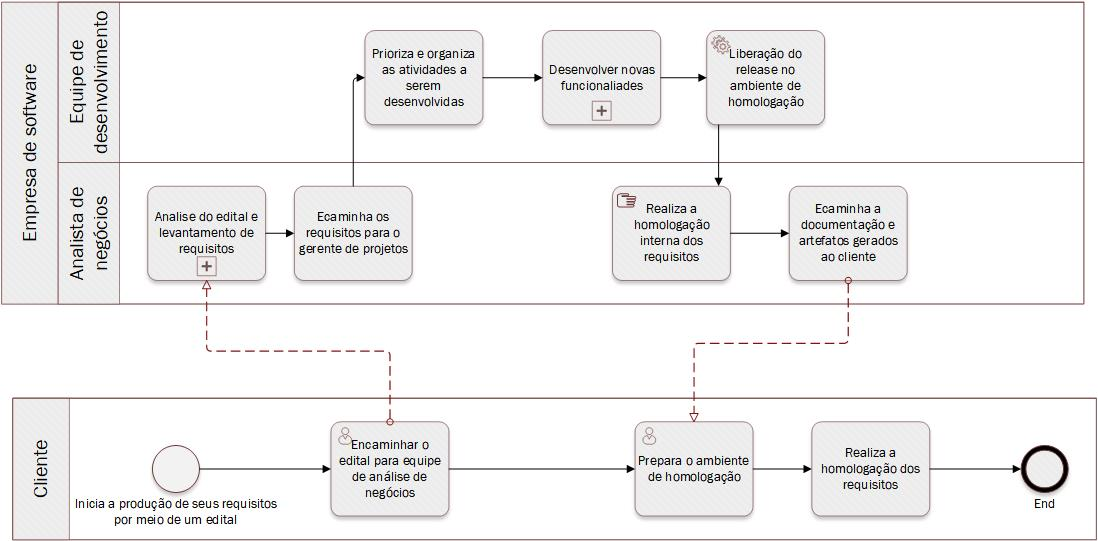
\includegraphics[width=\textwidth]{processo_de_software_BPMN1}
	\caption{Visão geral do processo de software}
\end{figure}

\begin{figure}
	\centering
	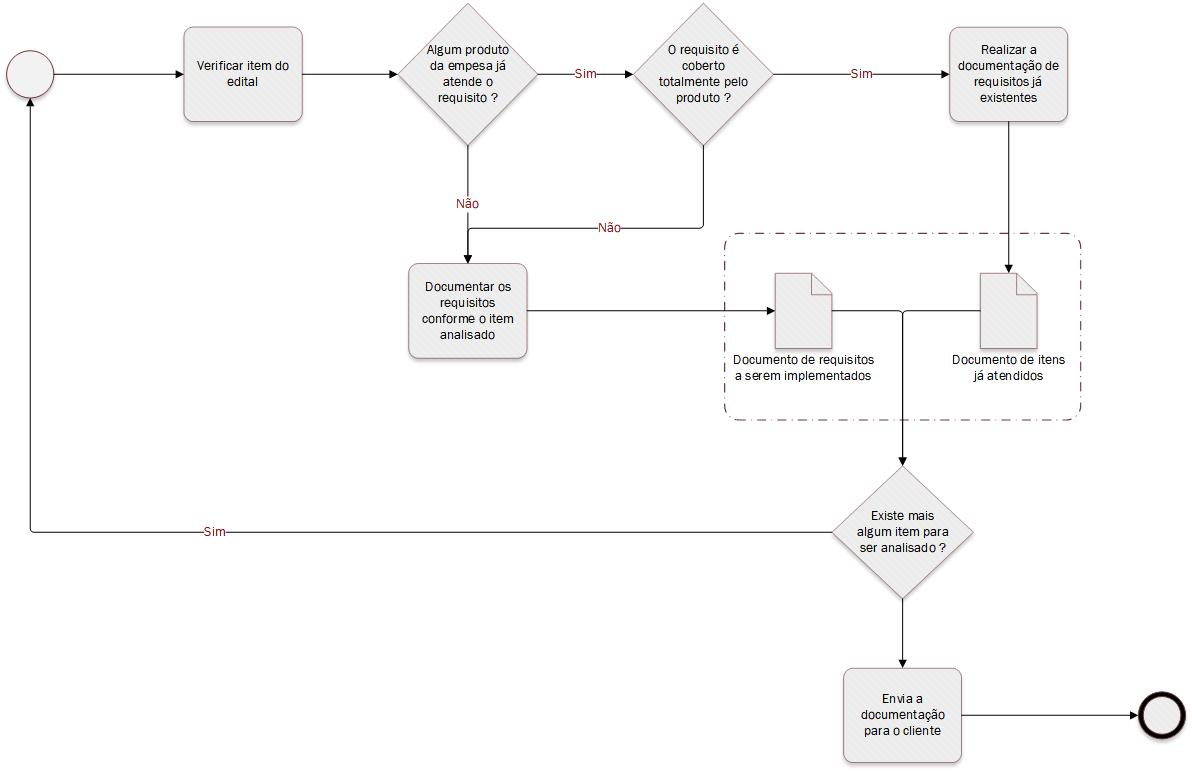
\includegraphics[width=\textwidth]{processo_de_software_BPMN2}
	\caption{Visão detalhada da etapa de análise de negócio}
\end{figure}

\begin{figure}
	\centering
	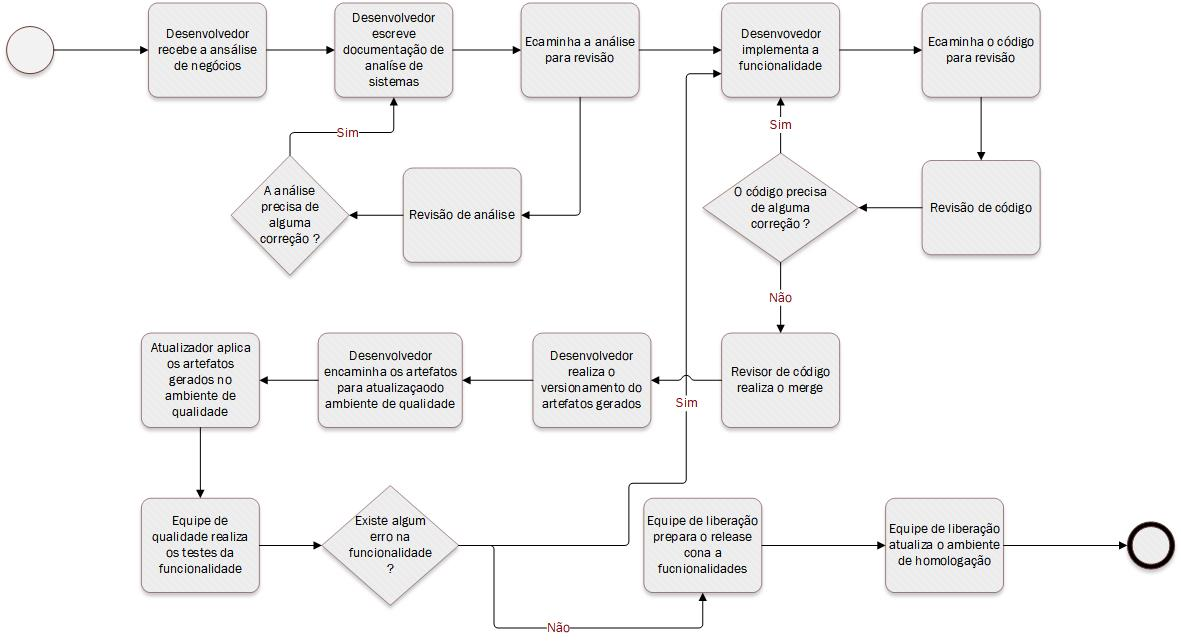
\includegraphics[width=\textwidth]{processo_de_software_BPMN3}
	\caption{Visão detalhada da etapa de desenvolvimento}
\end{figure}



\end{document}